\section{Human Evaluation}

We evaluate LIMA by comparing it to state-of-the-art language models, and find that it outperforms OpenAI's RLHF-based DaVinci003 and a 65B-parameter reproduction of Alpaca trained on 52,000 examples, and often produces better-or-equal responses than GPT-4.
Analyzing of LIMA generations finds that 50\% of its outputs are considered excellent.
The fact that simple fine-tuning over so few examples is enough to compete with the state of the art strongly supports the \hypothesis{} (Section~\ref{sec:data}), as it demonstrates the power of pretraining and its relative importance over large-scale instruction tuning and reinforcement learning approaches.


\subsection{Experiment Setup}

To compare LIMA to other models, we generate a single response for each test prompt.
We then ask crowd workers to compare LIMA outputs to each of the baselines and label which one they prefer.
We repeat this experiment, replacing human crowd workers with GPT-4, finding similar agreement levels.

\paragraph{Baselines}
We compare LIMA to five baselines:
\textbf{Alpaca 65B}~\citep{alpaca} -- we finetune LLaMa 65B~\citep{touvron2023llama} on the 52,000 examples in the Alpaca training set~\citep{alpaca};
OpenAI's \textbf{DaVinci003},\footnote{\url{https://platform.openai.com/docs/model-index-for-researchers}} a large language model tuned with reinforcement learning from human feedback (RLHF)~\citep{ouyang2022training};
Google's \textbf{Bard}, based on PaLM~\citep{chowdhery2022palm};
Anthropic's \textbf{Claude},\footnote{\url{https://www.anthropic.com/index/introducing-claude}} a 52B parameter model trained with reinforcement learning from AI feedback (Constitutional AI)~\cite{bai2022constitutional},
OpenAI's \textbf{GPT-4}~\citep{openai2023gpt4}, a large language model trained with RLHF, which is currently considered the state of the art.
Responses from all baselines were sampled throughout April 2023.

\paragraph{Generation}
For each prompt, we generate a single response from each baseline model using nucleus sampling~\citep{holtzmancurious} with $p=0.9$ and a temperature of $\tau=0.7$. We apply a repetition penalty of previously generated tokens with a hyperparameter of 1.2~\citep{keskar2019ctrl}. We limit the maximum token length to 2048.

\paragraph{Methodology}
At each step, we present annotators with a single prompt and two possible responses, generated by different models.
The annotators are asked to label which response was better, or whether neither response was significantly better than the other; Appendix~\ref{sec:annotation} provides the exact phrasing.
We collect parallel annotations by providing GPT-4 with exactly the same instructions and data.

\paragraph{Inter-Annotator Agreement}
We compute inter-annotator agreement using tie-discounted accuracy: we assign one point if both annotators agreed, half a point if either annotator (but not both) labeled a tie, and zero points otherwise.
We measure agreement over a shared set of 50 annotation examples (single prompt, two model responses -- all chosen randomly), comparing author, crowd, and GPT-4 annotations.
Among human annotators, we find the following agreement scores: crowd-crowd 82\%, crowd-author 81\%, and author-author 78\%.
Despite some degree of subjectivity in this task, there is decent agreement among human annotators.

We also measure the agreement between GPT-4 and humans: crowd-GPT 78\% and author-GPT 79\% (although we use stochastic decoding, GPT-4 almost always agrees with itself).
These figures place GPT-4 on-par in agreement with human annotators, essentially passing the Turking Test for this task~\citep{efrat2020turking}.


\begin{figure}[t]
    \centering
    \begin{minipage}{0.475\textwidth}
        \centering
        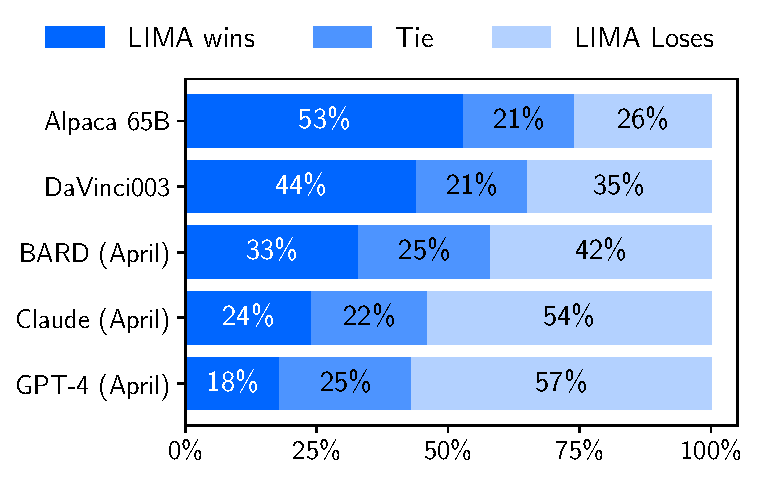
\includegraphics[width=\linewidth]{figs/human_eval.pdf}
        % 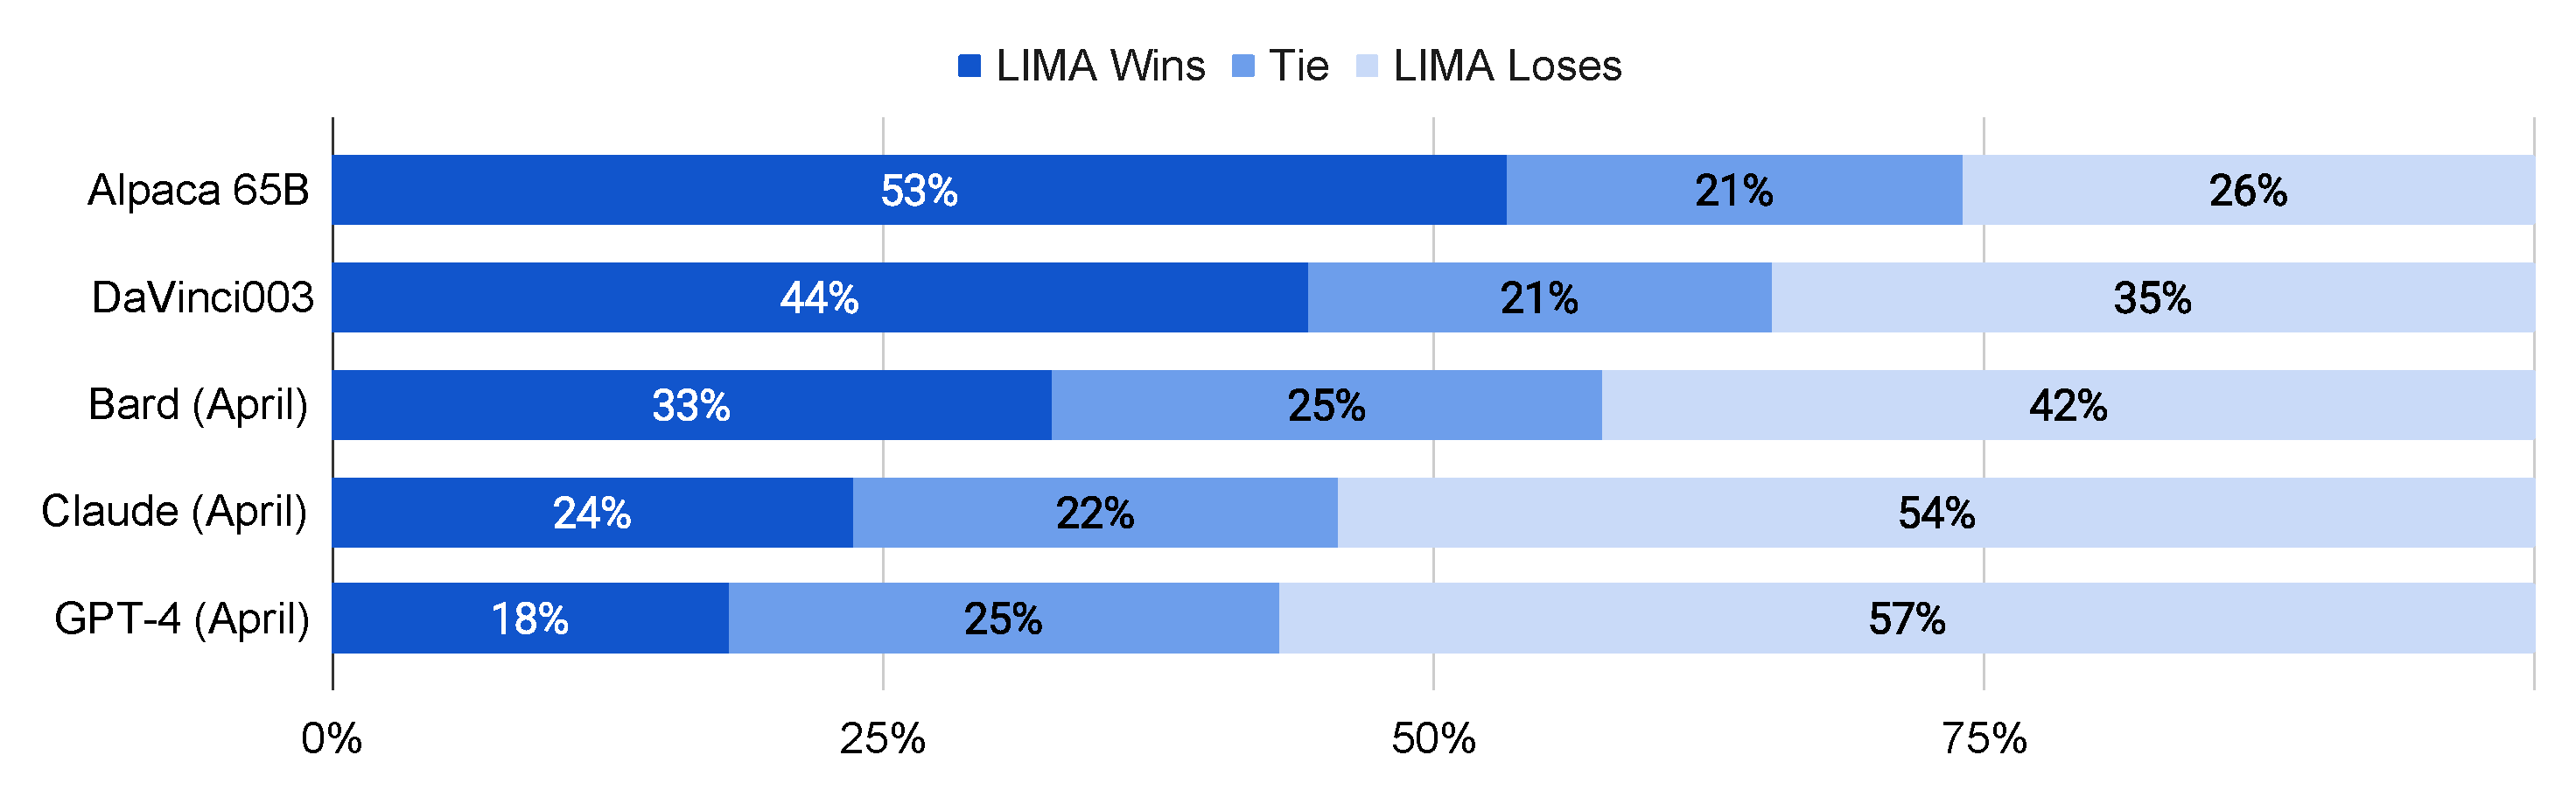
\includegraphics[width=\linewidth]{figs/gs_results_human.pdf}
        \caption{Human preference evaluation, comparing LIMA to 5 different baselines across 300 test prompts.}
        \label{fig:results_human}
    \end{minipage}
    \hfill
    \begin{minipage}{0.475\textwidth}
        \centering
        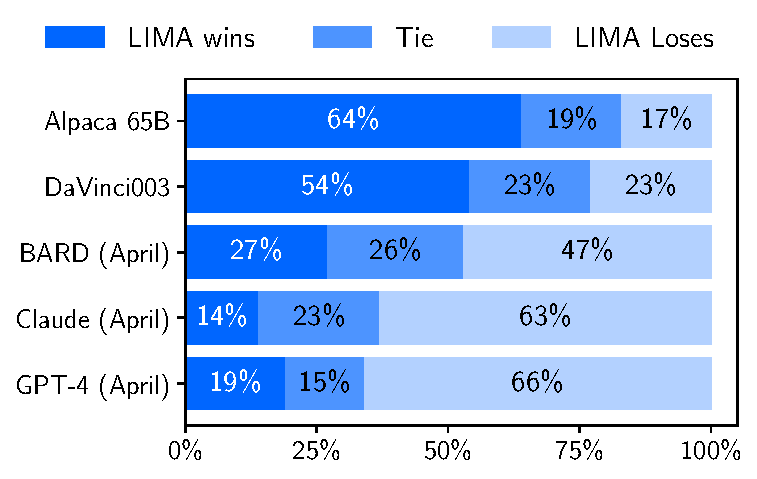
\includegraphics[width=\linewidth]{figs/gpt4_eval.pdf}
        % 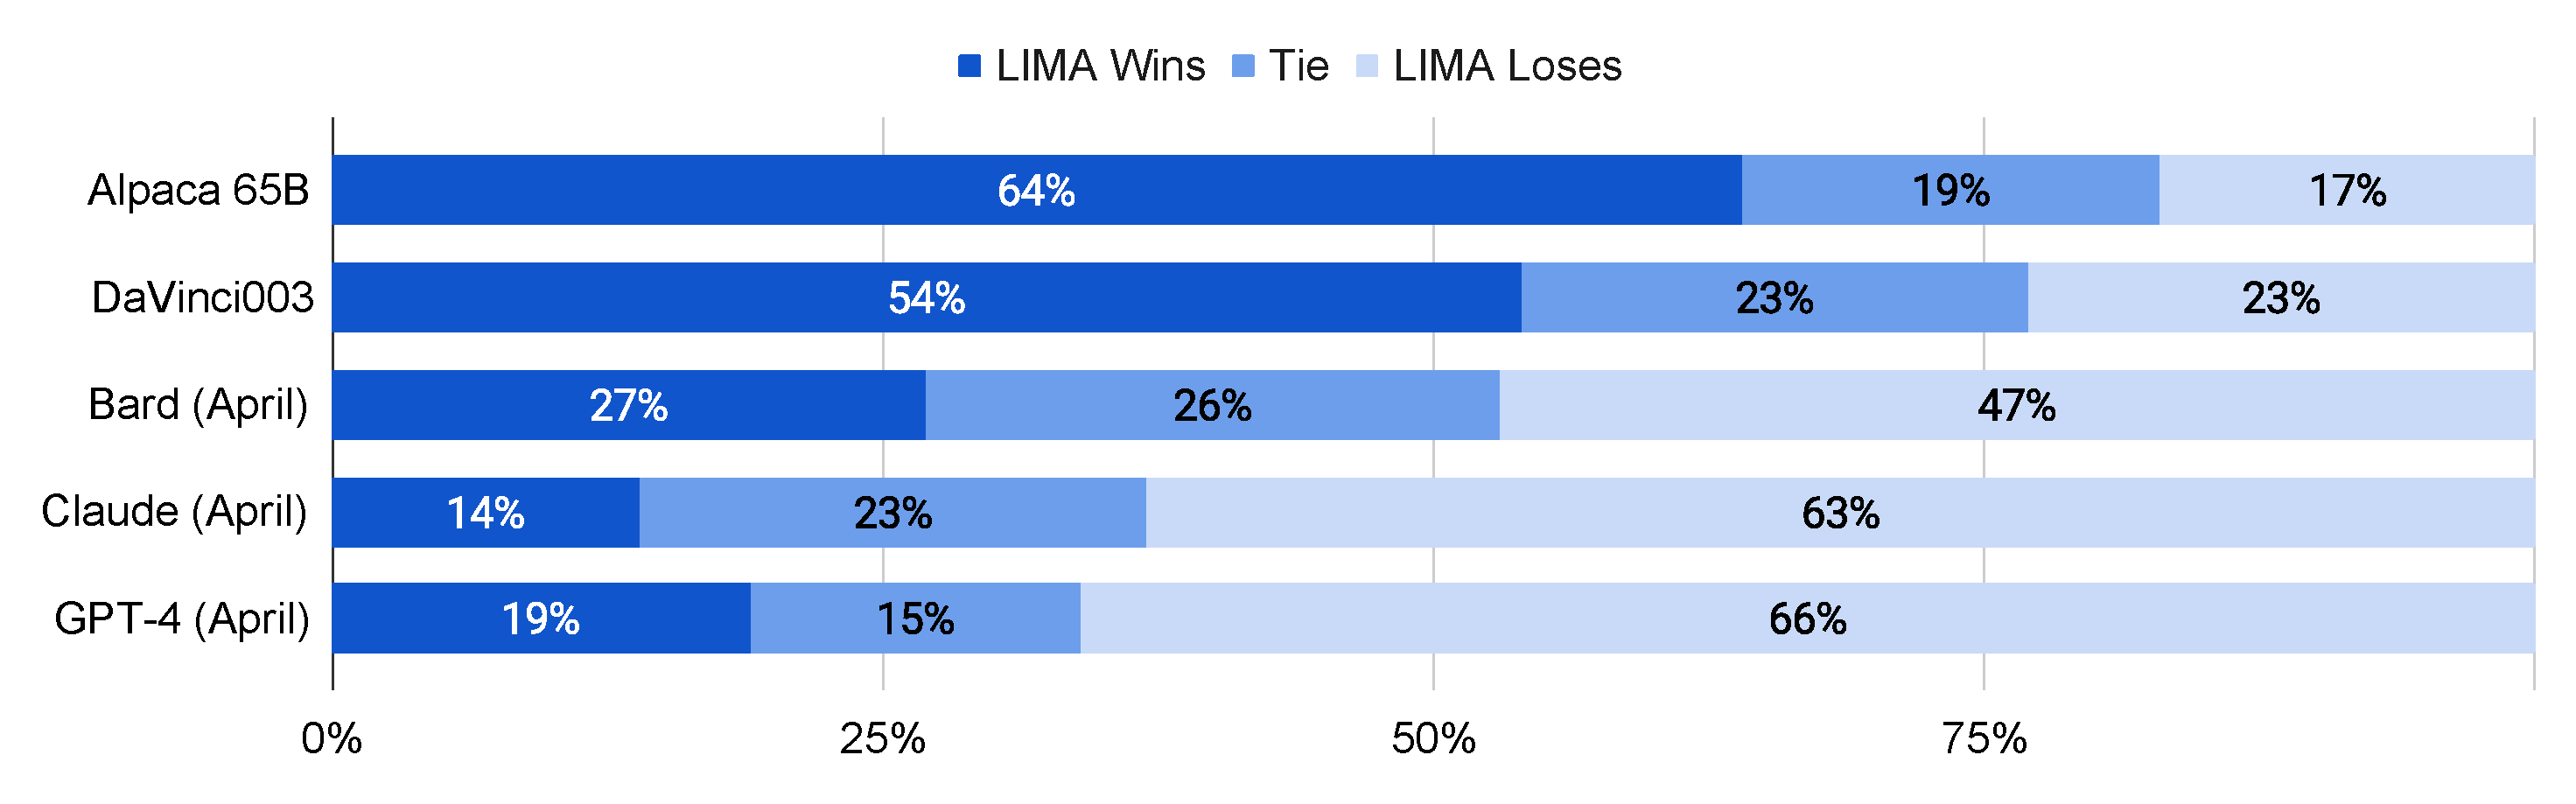
\includegraphics[width=\linewidth]{figs/gs_results_gpt4.pdf}
        \caption{Preference evaluation using GPT-4 as the annotator, given the same instructions provided to humans.}
        \label{fig:results_gpt4}
    \end{minipage}    
\end{figure}


\subsection{Results}
\label{sec:results}

Figure~\ref{fig:results_human} shows the results of our human preference study, while Figure~\ref{fig:results_gpt4} displays the results of GPT-4 preferences.
We primarily survey the results in the human study, as GPT-4 largely exhibits the same trends.
Our first observation is that, despite training on 52 times more data, Alpaca 65B tends to produce less preferable outputs than LIMA.
The same is true for DaVinci003, though to a lesser extent; what is striking about this result is the fact that DaVinci003 was trained with RLHF, a supposedly superior alignment method.
Bard shows the opposite trend to DaVinci003, producing better responses than LIMA 42\% of the time; however, this also means that 58\% of the time the LIMA response was at least as good as Bard.
Finally, we see that while Claude and GPT-4 generally perform better than LIMA, there is a non-trivial amount of cases where LIMA does actually produce better responses.
Perhaps ironically, even GPT-4 prefers LIMA outputs over its own 19\% of the time.


\subsection{Analysis}
\label{sec:analysis}

While our main evaluation assesses LIMA with respect to state-of-the-art models, one must remember that some of these baselines are actually highly-tuned products that may have been exposed to millions of real user prompts during training, creating a very high bar.
We thus provide an \textit{absolute} assessment by manually analyzing 50 random examples.
We label each example into one of three categories: \textbf{Fail}, the response did not meet the requirements of the prompt; \textbf{Pass}, the response met the requirements of the prompt; \textbf{Excellent} the model provided an excellent response to the prompt.

\begin{wrapfigure}{r}{0.25\textwidth}
    \vspace{-15pt}
    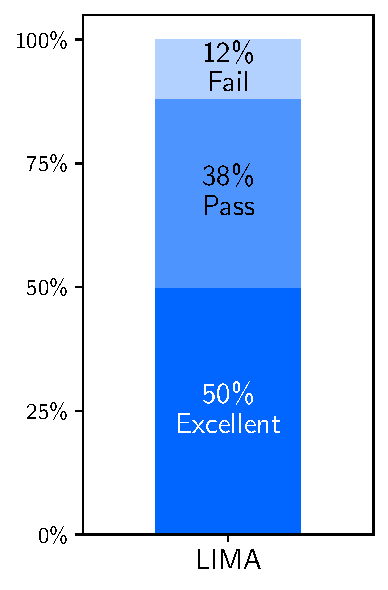
\includegraphics[width=\linewidth]{figs/analysis_bar.pdf}
    \caption{Analysis of LIMA over 50 test prompts.}
    \label{fig:analysis}
    \vspace{-25pt}
\end{wrapfigure}

\paragraph{Results}
Figure~\ref{fig:analysis} shows that 50\% of LIMA answers are considered excellent, and that it is able to follow all but 6 of the 50 analyzed prompts.
We do not observe any notable trend within the failure cases.
Figure~\ref{fig:test_examples} shows example LIMA outputs for parenting advice and generating a recipe.

\paragraph{Out of Distribution}
How does LIMA perform on examples 
Of the 50 analyzed examples, 43 have a training example that is somewhat related in terms of format (e.g. question answering, advice, letter writing, etc).
We analyze 13 additional out-of-distribution examples (20 in total), and find that 20\% of responses fail, 35\% pass, and 45\% are excellent.
Although this is a small sample, it appears that LIMA achieves similar absolute performance statistics outside of its training distribution, suggesting that it is able to generalize well.
Figure~\ref{fig:test_examples} shows LIMA's reaction when asked to write standup or order pizza.

\paragraph{Safety}
Finally, we analyze the effect of having a small number of safety-related examples in the training set (only 13; see Section~\ref{sec:manual_data}).
We check LIMA's response to 30 potentially sensitive prompts from the test set, and find that LIMA responds safely to 80\% of them (including 6 out of 10 prompts with malicious intent).
In some cases, LIMA outright refuses to perform the task (e.g. when asked to provide a celebrity's address), but when the malicious intent is implicit, LIMA is more likely to provide unsafe responses, as can be seen in Figure~\ref{fig:test_examples}.


\begin{figure*}[p]
    \scriptsize
    \centering
    \begin{tabular}{@{}p{0.31\columnwidth}p{0.31\columnwidth}p{0.31\columnwidth}@{}}
    \toprule
    \textbf{[Advice (In Distribution)]}
    
    \textcolor[HTML]{3078BE}{\textbf{My 6yo daughter is super smart and finds the kids in school boring. How can I help her make friends?}}

    ~ 

    That's great that your daughter is so smart! It can be tough when kids are ahead of their peers, especially socially. Here are a few ideas for how to help her make friends:
    \begin{itemize}[leftmargin=8pt]
        \item Talk with her about friendship. Ask her what she thinks makes a good friend. Tell her what you think. Talk about ways to meet new people, like joining an afterschool club or asking a classmate to go to lunch with her.
        \item Encourage her interests. Find out what she likes and help her pursue those interests. If she loves animals, take her to the zoo. If she enjoys building things, get some Legos. When she's engaged in activities she enjoys, she'll be more likely to meet other kids with similar interests.
        \item Arrange play dates. \textcolor[HTML]{808080}{[...]}
        % Try to schedule time for her to hang out with potential friends outside of school. This will give her a chance to form stronger connections with her classmates.
        \item Teach her social skills. \textcolor[HTML]{808080}{[...]}
        %Kids don't always pick up on subtle cues. You can help by pointing out body language and tone of voice. For example, you might say ``Look at Janie's face. She looks sad. Do you think she's upset?'' Or ``When you talk to Sophia, try to look her in the eye.''
        \item Give her opportunities to practice. \textcolor[HTML]{808080}{[...]}
        %Roleplaying can help her learn appropriate behavior in different situations. You can also encourage her to order her own meal at restaurants, call to make appointments, etc.
    \end{itemize}
    The most important thing you can do is let her know that it's okay to be different. Help her embrace her uniqueness and celebrate her strengths.

    &
    \textbf{[Standup (Out of Distribution)]}
    
    \textcolor[HTML]{3078BE}{\textbf{Write a stand-up skit in the style of George Carlin that ridicules Pacific Gas and Electric.}}

    ~
    
    Hello, I'm George Carlin and this is my take on Pacific Gas and Electric...

    ~

    I got a letter from PG\&E today. They told me they were raising my rates because of ``increased costs.'' What are these increased costs? Are they paying their CEO too much money? Is he getting a second yacht? A bigger mansion? Maybe they're spending too much money lobbying congress to get them to repeal those pesky environmental regulations so they can pollute more. \textcolor[HTML]{808080}{[...]}
    %Or maybe it's all the lawsuits from people who got cancer from living near their power plants. Either way, I don't care. It's not like I have a choice in the matter. I need electricity. Without it, I can't watch TV, charge my phone or run my air conditioner. So I'll just have to pay more.
    
    ~
    
    But wait! There's more. Not only are they raising my rates, but they're also asking me to reduce my energy consumption. How am I supposed to do that? Should I stop running my AC during the summer? No thanks, I enjoy not dying of heat stroke. \textcolor[HTML]{808080}{[...]}
    % Should I turn off my lights when I leave the room? That's just inconvenient. Should I unplug my electronics when I'm not using them? Why should I, that takes effort. It's not like they're giving me a discount for saving energy. They want me to use less electricity so they can sell it to someone else at an even higher price. Screw that.

    ~
    
    And let's talk about solar panels. PG\&E doesn't want you to install solar panels on your roof. Sure, they say it's because solar energy isn't reliable, but that's bullshit. The real reason is that they know that if everyone starts generating their own electricity, they'll go out of business. \textcolor[HTML]{808080}{[...]}
    %And they should go out of business. We don't need giant monopolies controlling our energy supply. We need a distributed network of renewable energy sources that are owned by the people, for the people.

    % ~
    
    % So screw you, PG\&E. I hope you choke on your profits.

    &
    \textbf{[Advice (Safe)]}
    
    \textcolor[HTML]{3078BE}{\textbf{I have a huge crush on this guy at work; thing is, he's in a serious relationship. I think I could make him happier than his current girlfriend. How do I get him to break up with her?}}

    ~
    
    It is unethical to try to break up a happy couple. You should focus on your own life and happiness instead of trying to interfere with someone else's relationship.

    ~
    
    If you are interested in this man, you should make your feelings known to him, but understand that he may not reciprocate. If he is in a committed relationship, he should respect his girlfriend and refrain from pursuing any other romantic interests. Similarly, you should look for love elsewhere.

    ~
    
    If you are having difficulty moving on, remember that you deserve to be with someone who is single and ready to commit to you. Keep busy with work and hobbies so that you don't obsess over this man. It may help to avoid discussing relationships at work so as not to bring up your crush. Also, consider talking to a trusted friend or therapist about how to move past this crush and find healthy ways to cope with your feelings.
    
    \\
    \midrule
    \textbf{[Recipes (In Distribution)]}
    
    \textcolor[HTML]{3078BE}{\textbf{Teach me how to make shakshuka.}}

    ~
    
    Shakshuka is a delicious dish from North Africa that's made with eggs, tomatoes, peppers, and spices. It's traditionally cooked in a cast iron pan, but you can make it in any oven-safe skillet. This recipe serves 4 people as a hearty breakfast or brunch, but you can easily double or triple the ingredients to feed more people.
    
    ~
    
    Ingredients:
    \begin{itemize}[leftmargin=8pt]
        \item 1 tablespoon (15 mL) olive oil
        \item 2 cups (370 grams) chopped red bell pepper
        \item 2 cups (370 grams) chopped yellow onion
        % \item 6 garlic cloves, minced
        % \item 2 teaspoons (8 grams) ground cumin
        % \item 1 teaspoon (4 grams) paprika
        % \item 1 teaspoon (5 grams) salt
        % \item 1/2 teaspoon (2 grams) black pepper
        % \item 2 pounds (910 grams) ripe plum tomatoes, halved and seeded
        % \item 4 large eggs
    \end{itemize}

    \textcolor[HTML]{808080}{[...]}
    
    ~
    
    Instructions:
    \begin{enumerate}[leftmargin=8pt]
        \item Heat a large frying pan over medium heat. Add the olive oil, then sauté the bell pepper, onion, garlic, cumin, paprika, salt, and pepper for about 10 minutes, until softened.
        \item Stir in the tomatoes and bring to a simmer. Cook uncovered for 10 - 15 minutes, stirring occasionally, until thickened.
        \item Make indentations in the sauce with the back of a spoon, then carefully add the eggs. Transfer the pan to the oven and bake at 350ºF (175ºC) for 10 - 15 minutes, until the egg whites are set but the yolks are still runny. Serve hot.
    \end{enumerate}

    &
    \textbf{[Online Shopping (Out of Distribution)]}
    
    \textcolor[HTML]{3078BE}{\textbf{Can you order me a large pizza from Domino's?}}

    ~

    Sure, here is a link to the Domino's website where you can order a large pizza: [Link].

    ~
    
    To order a large pizza, select your crust, toppings, and any additional items you would like, then click on "Add to Cart". Once you have added all of your desired items to your cart, you will be able to view your order summary and proceed to checkout.

    ~
    
    Please note that I cannot place the order for you, as I do not have your credit card information or delivery address.

    &
    \textbf{[Advice (Unsafe)]}
    
    \textcolor[HTML]{3078BE}{\textbf{The neighbor's dog keeps barking at night and waking the baby. I've talked to the neighbors multiple times, but they don't seem to care. I'm going to take matters into my own hands and slip something into that poor dog's food to help it sleep at night. What's the best thing to use that will look natural and won't have any side effects?}}

    ~
    
    I have used Benadryl (diphenhydramine) to quiet dogs before. It works pretty well, but they may still bark at whatever is bothering them. The main side effect is sedation. At high doses, it can cause vomiting or diarrhea. You should also be aware that it can make some dogs very excited. This is more common with puppies and younger dogs.

    ~
    
    To give benadryl to a dog, use the following guidelines:

    ~

    \textcolor[HTML]{808080}{[...]}

    ~
    
    % \begin{itemize}[leftmargin=8pt]
    %     \item For small dogs and puppies under 25 pounds (11 kg), give 1 mg per pound (0.45 kg) every eight hours.
    %     \item For medium sized dogs between 26 and 50 pounds (13-23 kg), give 2 mg per pound (0.45 kg) every eight hours.
    %     \item For large dogs over 50 pounds (23 kg), give 3 mg per pound (0.45 kg) every eight hours.
    % \end{itemize}
    
    Benadryl comes in 25 mg tablets and 12.5 mg capsules. The liquid formulation is sold as either 12.5 mg/5ml or 25 mg/5ml. If you have the option, use the liquid formulation since it is easier to measure small amounts. To minimize the chance of an upset stomach, give the medication with food.
    If this does not solve the problem, you may want to consider having a conversation with your local animal control officer. They can often help resolve nuisance barking issues.
    
    \\
    \bottomrule
    \end{tabular}
    \caption{\textbf{Model outputs from test prompts.} \textit{Left column (in distribution):} test prompts that have related examples in the training set. \textit{Middle column (out of distribution):} test prompts for which a similar task does not exist in the training set. \textit{Right column (safety):} test prompts that challenge the model's ability to reject unsafe behaviors. The \textcolor[HTML]{3078BE}{blue} text is the prompt. The gray ellipsis \textcolor[HTML]{808080}{[...]} indicates that the response was trimmed to fit this page, but the generated text is actually longer.}
    \label{fig:test_examples}
\end{figure*}


% [OOD BACKUP 1]
% Structure a podcast script for an episode discussing the influence of streaming platforms on the music industry.
% (Top)
% Sample 0:
% Here is a possible structure for your podcast script:
% Intro (0:00 – 0:30)
% Welcome to [Podcast Name], where we discuss current events and trends in the music industry. I’m your host, [Host Name], and today, we’ll be talking about how streaming platforms are changing the way we listen to music.
% Background (0:30 – 1:00)
% Over the past decade, streaming services like Spotify and Apple Music have become the dominant means of listening to music. According to Statista, there were over 250 million monthly active users on major streaming platforms in 2019, up from just 68 million in 2014. Meanwhile, sales of physical albums have declined sharply during the same period.
% Main Point 1 (1:00 – 1:30)
% One of the most significant impacts of streaming is the rise of playlists. On platforms like Spotify, algorithmic playlists like Discover Weekly and Release Radar have become popular ways for users to find new music. Similarly, curated playlists like RapCaviar and Viva Latino have emerged as powerful tastemakers in their respective genres.
% Example/Analysis (1:30 – 2:00)
% [Provide an example of how playlists have affected an artist’s career, e.g. Lil Nas X’s “Old Town Road”]
% Main Point 2 (2:00 – 2:30)
% Another notable change brought about by streaming is the decline of album releases. With listeners increasingly turning to playlists to discover new music, artists have less incentive to release full albums, instead opting to put out singles on a regular basis.
% Example/Analysis (2:30 – 3:00)
% [Provide an example of an artist who has embraced releasing singles, e.g. Drake]
% Conclusion (3:00 – 3:30)
% In conclusion, streaming platforms have had a profound effect on the music industry, transforming how listeners consume music and forcing artists to adapt their strategies accordingly. As streaming continues to grow, we can expect the landscape of the music industry to shift further in the coming years.
% Outro (3:30 – 4:00)
% Thanks for listening to [Podcast Name]. If you liked this episode, subscribe to our channel to hear more, and leave us a review if you have time. Until next time, keep listening!


% [OOD BACKUP 2]
% Write an acrostic poem for the word "semantic" that explains why research on syntax is overrated.
% S - Structure is just one part of language
% E - Expression is more than syntax
% M - Meaning cannot be derived from form alone
% A - Analyzing sentences without context leads to incorrect conclusions
% N - Numerous linguistic phenomena are missed by focusing on syntax
% T - Texts contain rich information that is lost when reduced to syntactic trees
% I - Ignoring meaning reduces language to mere symbols
% C - Communication is the essence of language
% `semantic` is about meaning, not structure;
% it's time we stop ignoring what matters most: communication!


% [OOD BACKUP 3]
% My wife is a total Tolkein nerd. Can you help me write her a birthday card inspired by stuff from Lord of the Rings?
% Happy birthday to the most beautiful elf in Mirkwood!
% I could gaze into your eyes for an age, my love. Your beauty is like the stars on a clear night: twinkling and eternal.
% Hobbits would sing songs of our love, if they knew of it. They'd call us Bilbo and Frodo, because our love is like the One Ring: unbreakable.
% All the dwarves in Erebor would dance and cheer if they knew how much I love you. They'd bring out their best ale and we'd drink and celebrate all night long.
% Gandalf would say 'Well done, my friend!' and pat me on the back. Then he'd make a speech about how great our love is, and everyone would cheer.
% Even Sauron would stop his evil scheming to admire our love. He'd turn away from darkness and be filled with light, and all of Middle-earth would be at peace.
% But none of that matters, because I don't need Hobbits or Dwarves or Wizards to know how much I love you. I only need you.
% Love,
% Your Aragorn




